\documentclass[11pt,a4paper]{article}

% Pacchetti di base 
\usepackage[utf8]{inputenc} % caratteri speciali
\usepackage[T1]{fontenc} 
\usepackage[italian]{babel} % Adattamento all'italiano
\usepackage{lmodern} % resa grafica 
\usepackage[a4paper,margin=2.5cm]{geometry} % margini

% Matematica 
\usepackage{amsmath,amssymb}

% Tabelle e figure 
\usepackage{booktabs} % estetica 
\usepackage{graphicx}
\usepackage{float} % posizionamento delle figure e tabelle
\usepackage{caption} % didascalie di figure e tabelle

% Collegamenti ipertestuali 
\usepackage{hyperref} % possibilit\`{a} di cliccare riferimenti
\hypersetup{
    colorlinks=true,
    linkcolor=black,
    urlcolor=blue,
    citecolor=black
}

% Interlinea 
\usepackage{setspace}
\onehalfspacing

\title{Previsione dell'abbandono dei dipendenti:\\ un confronto tra modelli di classificazione}
\author{Valeria Di Stefano \and Margherita Marinelli \and Edoardo Moretti}
\date{Gruppo 9 --- Progetto del corso\\ Introduzione alla Data Science e al Pensiero Computazionale}

\begin{document}

\maketitle
% indice
\tableofcontents
\newpage


\section{Introduzione}

In questo lavoro viene analizzato il dataset \emph{Employee Attrition}, con l'obiettivo di costruire e confrontare diversi modelli di classificazione, in grado di prevedere se un dipendente lascer\`{a} l'azienda in cui lavora a partire da alcune caratteristiche demografiche, contrattuali e lavorative.

Il report \`{e} strutturato come segue: nella Sezione~\ref{sec:dataset} vengono descritte le caratteristiche principali del dataset e le relazioni tra alcune variabili ritenute significative; nella Sezione~\ref{sec:metodologia} viene descritto com'\`{e} stato rielaborato il dataset e quali modelli di classificazione sono stati utilizzati; nella Sezione~\ref{sec:risultati} vengono riportati i risultati ottenuti dai diversi modelli; nella Sezione~\ref{sec:discussione} vengono valutati e confrontati i risultati; nella Sezione~\ref{sec:conclusioni} vengono riassunte le conclusioni del lavoro.

Il notebook con tutte le analisi, il dataset, le figure e il presente report sono disponibili nel repository GitHub del progetto: 
\\
\url{https://github.com/margheritamarinelli/Progetto-Data-Science-gruppo-9} % (link del repository)


\section{Dataset}
\label{sec:dataset}

Il dataset \`{e} composto da 1470 osservazioni (dipendenti) e 35 variabili, di cui 26 numeriche e 9 categoriche. Non sono presenti n\'{e} valori mancanti n\'{e} outliers. La variabile target, \texttt{Attrition}, indica se un dipendente ha abbandonato (\texttt{Yes}) o meno (\texttt{No}) l'azienda.

\subsection{Variabili non informative}
\label{sec:non-informative}

Dall'analisi sono emerse alcune variabili prive di valore informativo, in quanto costanti per tutte le osservazioni o puramente identificative: \texttt{EmployeeCount}, \texttt{StandardHours}, \texttt{Over18} ed \texttt{EmployeeNumber}. Tali variabili presentano correlazione di Pearson non calcolabile (\texttt{NaN}) poich\'{e} a varianza nulla e sono state rimosse prima della fase di modellazione.

\subsection{Squilibrio delle classi}

Una caratteristica fondamentale del dataset, che condiziona tutte le scelte metodologiche successive, \`{e} il forte squilibrio tra le classi della variabile target: l'83,88\% dei dipendenti rimane in azienda, mentre solo il 16,12\% abbandona. Questo squilibrio rende l'accuratezza una metrica poco informativa, per questo \`{e} stata affiancata da altre metriche (precision, recall e f1-score) ed \`{e} stato utilizzato il parametro \texttt{class\_weight = 'balanced'} nei modelli.

\subsection{Relazioni tra variabili}

Per comprendere meglio la struttura del dataset e individuare possibili fattori associati all'abbandono dei dipendenti, sono state analizzate le relazioni tra alcune variabili numeriche e categoriche mediante grafici esplorativi e misure di correlazione.

Dalla \emph{Heatmap} risulta che ci siano pochi valori di correlazione positiva forte:
\begin{itemize}
    \item \texttt{JobLevel} e \texttt{MonthlyIncome};
    \item \texttt{TotalWorkingYears} e \texttt{JobLevel};
    \item \texttt{YearsAtCompany} e \texttt{YearsWithCurrManager};
    \item \texttt{YearsAtCompany} e \texttt{YearsInCurrentRole}.
\end{itemize}
Queste relazioni sono coerenti con il contesto aziendale: dipendenti con maggiore esperienza tendono ad occupare posizioni gerarchiche pi\`{u} elevate e ad avere retribuzioni maggiori.

\begin{figure}[H]
    \centering
    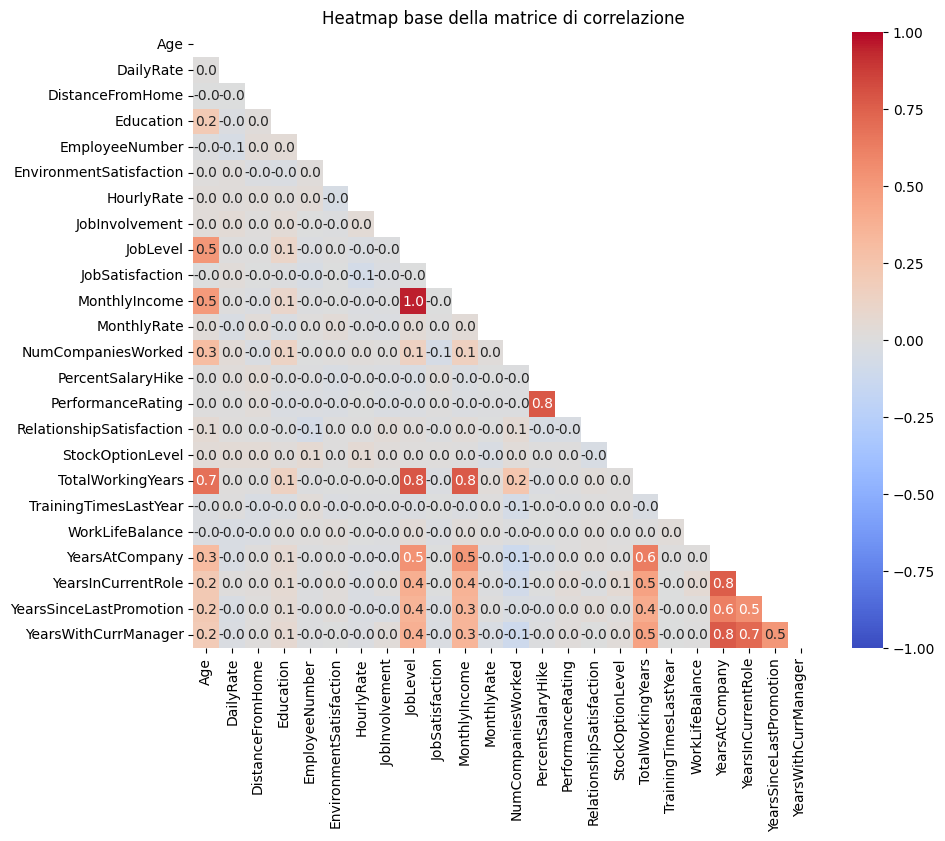
\includegraphics[width=0.9\textwidth]{immagini/Heatmap_progetto.png}
    \caption{Heatmap delle correlazioni tra le variabili numeriche.}
    \label{fig:heatmap}
\end{figure}

L'analisi grafica mostra che la probabilit\`{a} di abbandono non \`{e} uniforme tra i diversi gruppi di lavoratori. I dipendenti che effettuano straordinari presentano una quota di abbandono sensibilmente superiore rispetto a coloro che non svolgono lavoro straordinario. Questo suggerisce che un carico di lavoro elevato possa contribuire all'insoddisfazione e alla decisione di lasciare l'azienda.

Analogamente, i dipendenti pi\`{u} giovani e con minore anzianit\`{a} aziendale mostrano una maggiore propensione all'abbandono rispetto ai lavoratori pi\`{u} esperti.

I boxplot e gli istogrammi evidenziano distribuzioni spesso asimmetriche, soprattutto per le variabili legate all'esperienza lavorativa e alla permanenza in azienda. Sono presenti alcuni valori estremi in variabili come:
\begin{itemize}
    \item \texttt{TotalWorkingYears};
    \item \texttt{YearsAtCompany};
    \item \texttt{YearsSinceLastPromotion}.
\end{itemize}
Tali osservazioni rappresentano tuttavia casi plausibili e coerenti con il contesto aziendale e non sono state considerate come anomalie o errori nei dati.


\section{Metodologia}
\label{sec:metodologia}

\subsection{Rielaborazione dei dati}

Prima della fase di modellazione, il dataset \`{e} stato sottoposto alle seguenti operazioni:
\begin{itemize}
    \item Rimozione delle variabili non informative (Sezione~\ref{sec:non-informative});
    \item Conversione della variabile target in formato binario (\texttt{No} $\rightarrow$ 0, \texttt{Yes} $\rightarrow$ 1);
    \item One-hot encoding delle altre variabili categoriche;
    \item Suddivisione del dataset in training set (70\%) e test set (30\%), con stratificazione sulla variabile target per mantenerne le proporzioni sia nel training set che nel test set;
    \item Standardizzazione delle feature numeriche nei modelli di Regressione Logistica e k-NN.
\end{itemize}

\subsection{Modelli}

Sono stati addestrati tre modelli di classificazione:

\paragraph{Regressione Logistica.} Stima la probabilit\`{a} di appartenenza ad una classe mediante la funzione sigmoide:
\begin{equation}
    \sigma(z) = \frac{1}{1 + e^{-z}}, \qquad z = \beta_0 + \sum_{i=1}^{p} \beta_i x_i .
\end{equation}
Il modello \`{e} stato addestrato inizialmente con una soglia pari a 0,5 e poi con una soglia pari a 0,7.

\paragraph{k-NN (Nearest Neighbors).} Classifica una nuova osservazione in base alla classe predominante tra i $k$ vicini pi\`{u} prossimi nello spazio delle feature. Sono stati testati $k = 5$ e $k = 3$.

\paragraph{Random Forest.} Combina numerosi alberi decisionali e produce la classificazione finale mediante voto maggioritario. Questo approccio consente di catturare relazioni non lineari e di stimare l'importanza delle variabili. Sono stati utilizzati 100 alberi.

\subsection{Valutazione dei modelli}

Per ciascun modello sono state calcolate le seguenti metriche sul test set: accuratezza, precision, recall, F1-score e matrice di confusione. Per ottenere stime pi\`{u} robuste, e meno sensibili alla particolare suddivisione del dataset in training e test set, le configurazioni finali dei tre modelli sono state valutate mediante una procedura di 10-fold stratified cross-validation, che preserva la distribuzione della variabile target in ciascuna partizione dei dati.


\section{Risultati}
\label{sec:risultati}

\subsection{Analisi esplorativa}

L'analisi esplorativa svolta nelle sezioni precedenti ha evidenziato la presenza di alcune caratteristiche potenzialmente rilevanti per la previsione dell'abbandono. In particolare, variabili legate all'esperienza lavorativa, all'anzianit\`{a} aziendale, alla retribuzione e agli straordinari mostrano associazioni significative con la variabile target.

Le relazioni osservate suggeriscono che il fenomeno dell'abbandono non dipenda da un singolo fattore, ma dall'interazione di diversi aspetti della carriera e delle condizioni di lavoro dei dipendenti. Tali evidenze hanno motivato l'utilizzo di modelli di classificazione capaci di combinare simultaneamente tutte le informazioni disponibili.

Inoltre, la presenza di uno squilibrio marcato tra le classi ha evidenziato la necessit\`{a} di valutare i modelli mediante metriche pi\`{u} informative della sola accuratezza, ponendo particolare attenzione alla capacit\`{a} di identificare correttamente i dipendenti che lasciano l'azienda.

\subsection{Interpretazione dei modelli}

Nel caso della Regressione Logistica, l'analisi dei coefficienti ha permesso di identificare le feature che contribuiscono maggiormente all'aumento o alla diminuzione della probabilit\`{a} di abbandono. In particolare, la presenza di straordinari risulta associata ad una maggiore probabilit\`{a} di abbandono, mentre livelli pi\`{u} elevati di anzianit\`{a} aziendale e di esperienza lavorativa tendono ad essere associati ad una minore probabilit\`{a} di lasciare l'azienda.

Tali dinamiche trovano riscontro visivo nei grafici, dove l'analisi dei punti classificati erroneamente evidenzia come nessuna singola variabile \`{e} sufficiente a spiegare completamente il fenomeno.

Per la Random Forest \`{e} stata invece analizzata l'importanza delle variabili (\emph{feature importance}). I risultati mostrano che fattori quali \texttt{MonthlyIncome}, \texttt{Age}, \texttt{TotalWorkingYears}, \texttt{YearsAtCompany} ed \texttt{OverTime} figurano tra le variabili pi\`{u} rilevanti per la classificazione. Tali risultati sono coerenti con quanto osservato durante l'analisi esplorativa e confermano il ruolo centrale dell'esperienza lavorativa, della retribuzione e del carico di lavoro nel fenomeno dell'abbandono.

Nel complesso, l'interpretazione dei modelli conferma che l'abbandono dei dipendenti non sia determinato da una singola caratteristica, ma dall'interazione di diversi aspetti legati all'esperienza professionale, alla soddisfazione lavorativa e alle condizioni di lavoro.

\subsection{Confronto tra modelli}

La Tabella~\ref{tab:test} riporta le metriche di valutazione sul test set per i tre modelli (Regressione Logistica a soglia 0,5, k-NN con $k=5$, Random Forest con 100 alberi).

\begin{table}[H]
    \centering
    \caption{Metriche di valutazione sul test set.}
    \label{tab:test}
    \begin{tabular}{lcccc}
        \toprule
        \textbf{Modello} & \textbf{Accuratezza} & \textbf{Precision} & \textbf{Recall} & \textbf{F1-score} \\
        \midrule
        Regressione Logistica & 0.76 & 0.36 & 0.68 & 0.47  \\
        k-NN ($k=5$)          & 0.84 & 0.50 & 0.07 & 0.12  \\
        Random Forest         & 0.83 & 0.43 & 0.08 & 0.14  \\
        \bottomrule
    \end{tabular}
\end{table}

Come si osserva, k-NN e Random Forest raggiungono un'accuratezza pi\`{u} elevata rispetto alla Regressione Logistica ma una recall estremamente bassa sulla classe minoritaria (7--8\%): ci\`{o} significa che questi modelli classificano quasi sempre i dipendenti come destinati a rimanere in azienda. La Regressione Logistica, pur con un'accuratezza inferiore, identifica correttamente circa il 68\% dei dipendenti che abbandonano effettivamente l'azienda.

\begin{table}[H]
    \centering
    \caption{Risultati della 10-fold stratified cross-validation (media ± deviazione standard).}
    \label{tab:cv}
    \begin{tabular}{lcccc}
        \toprule
        \textbf{Modello} & \textbf{Accuratezza} & \textbf{Precision} & \textbf{Recall} & \textbf{F1-score} \\
        \midrule
        Regressione Logistica & 0.76 (± 0.03) & 0.38 (± 0.04) & 0.75 (± 0.10) & 0.51 (± 0.06) \\
        k-NN ($k=5$)          & 0.85 (± 0.07) & 0.61 (± 0.30) & 0.15 (± 0.08) & 0.23 (± 0.12) \\
        Random Forest         & 0.86 (± 0.02) & 0.83 (± 0,23) & 0.16 (± 0.05) & 0.26 (± 0.08) \\
        \bottomrule
    \end{tabular}
\end{table}

I risultati della 10-fold cross-validation confermano questa tendenza: la Regressione Logistica mantiene una recall media solida, mentre k-NN e Random Forest restano fermi su valori di recall del 15--16\%, con deviazioni standard elevate sulla precision, segno di instabilit\`{a} nell'identificazione degli abbandoni.


\section{Discussione}
\label{sec:discussione}

\subsection{Punti di forza}

Uno dei principali punti di forza del lavoro \`{e} l'utilizzo di diverse metriche di valutazione, che ha permesso di evitare interpretazioni fuorvianti basate esclusivamente sull'accuratezza. Inoltre, il confronto tra modelli differenti ha consentito di analizzare il problema sia attraverso approcci lineari, sia attraverso modelli non lineari. La Regressione Logistica si \`{e} dimostrata particolarmente efficace nell'identificare i dipendenti che abbandonano l'azienda, ottenendo valori di recall significativamente superiori rispetto agli altri modelli. La cross-validation ha inoltre confermato la stabilit\`{a} di questo comportamento.

\subsection{Limiti}

Il principale limite dell'analisi \`{e} rappresentato dal forte sbilanciamento della variabile target. La ridotta numerosit\`{a} dei casi di abbandono rende pi\`{u} difficile l'apprendimento delle caratteristiche associate ad esso e porta alcuni modelli a privilegiare la classificazione della classe maggioritaria.

\subsection{Interpretabilit\`{a}}

Dal punto di vista dell'interpretabilit\`{a}, la Regressione Logistica offre il vantaggio di coefficienti direttamente interpretabili, che permettono di comprendere quali variabili contribuiscano ad aumentare o diminuire la probabilit\`{a} di abbandono. Anche la Random Forest offre un certo grado di interpretabilit\`{a} attraverso l'analisi della feature importance, pur non permettendo una lettura diretta delle relazioni tra variabili e predizione.

Al contrario, il modello k-NN presenta una minore interpretabilit\`{a}, poich\'{e} le decisioni vengono prese sulla base della vicinanza tra osservazioni, senza fornire indicazioni esplicite sul ruolo delle singole feature.


\subsection{Tipologia degli errori}

L'analisi delle matrici di confusione mostra che gli errori pi\`{u} frequenti riguardano i falsi negativi, ossia dipendenti che abbandonano realmente l'azienda ma che vengono classificati come destinati a rimanere. Questo tipo di errore risulta particolarmente rilevante dal punto di vista applicativo, poich\'{e} impedisce all'azienda di individuare in anticipo i lavoratori a rischio di abbandono.

Sotto questo aspetto, la Regressione Logistica si dimostra preferibile rispetto agli altri modelli, poich\'{e} riduce significativamente il numero di falsi negativi grazie a una recall pi\`{u} elevata.

\subsection{Costo computazionale}

Dal punto di vista computazionale, la Regressione Logistica rappresenta il modello pi\`{u} efficiente, richiedendo tempi di addestramento ridotti e una limitata complessit\`{a} computazionale. Il modello k-NN presenta invece un costo di addestramento molto basso, ma richiede il confronto con tutte le osservazioni del training set durante la fase di predizione.

La Random Forest \`{e} il modello pi\`{u} costoso dal punto di vista computazionale, poich\'{e} richiede la costruzione di numerosi alberi decisionali. I risultati ottenuti mostrano tuttavia che l'aumento della complessit\`{a} del modello non si traduce necessariamente in una migliore capacit\`{a} di identificare i dipendenti che abbandonano l'azienda.

\begin{figure}[H]
    \centering
    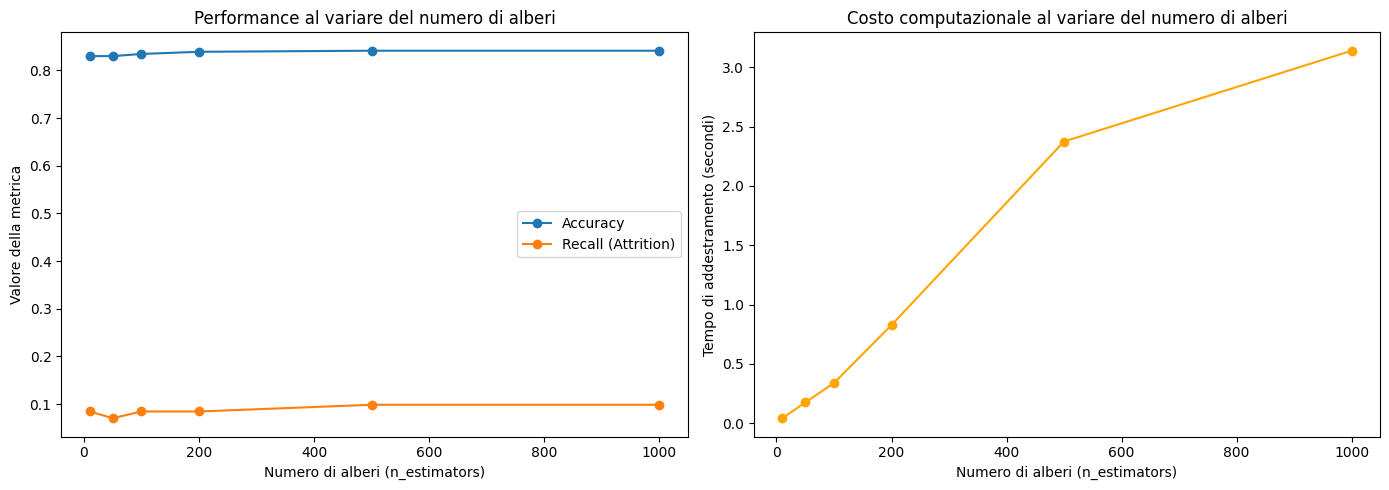
\includegraphics[width=1\textwidth]{immagini/Performance_RF.png}
    \caption{Confronto delle prestazioni dei modelli.}
    \label{fig:confronto}
\end{figure}


\section{Conclusioni}
\label{sec:conclusioni}

In questo progetto sono stati analizzati i dati del dataset \emph{Employee Attrition} con l'obiettivo di prevedere l'abbandono dei dipendenti mediante tre modelli di classificazione. L'analisi esplorativa ha evidenziato l'importanza di fattori quali et\`{a}, esperienza lavorativa, anzianit\`{a} aziendale, reddito e straordinari. I risultati dei tre modelli mostrano che l'accuratezza, considerata isolatamente, non rappresenta una metrica adeguata per questo problema a causa dello squilibrio tra le classi. Sebbene k-NN e Random Forest abbiano ottenuto valori di accuratezza pi\`{u} elevati, la Regressione Logistica ha dimostrato una capacit\`{a} nettamente superiore di identificare i dipendenti che abbandonano l'azienda, ottenendo i migliori valori di recall sia sul test set sia nella cross-validation.

Nel complesso, la Regressione Logistica rappresenta il miglior compromesso tra capacit\`{a} predittiva, robustezza, interpretabilit\`{a} e costo computazionale. L'analisi ha inoltre confermato che il fenomeno dell'abbandono dipende dall'interazione di molteplici fattori individuali e lavorativi, rendendo particolarmente importante l'utilizzo di strumenti quantitativi per supportare le decisioni aziendali.


\section{Riferimenti bibliografici}

\begin{thebibliography}{9}

    \bibitem{dataset}
    IBM HR Analytics Employee Attrition \& Performance Dataset.


\end{thebibliography}

\end{document}

